\newpage
\section{Level Converter}
The purpose of this block is to supply both the various 5 Volt components in the system. This is done by converting the 12 VDC from the Voltage Adaptor's output down.

\subsection{Design} \fxnote{Lyder meget som krav til konverteren, ikke design - JH}
In order to determine which component can be used to convert the voltage, the maximum current drawn by the 5 VDC components must be calculated. This is done by looking through the components' datasheets. It is assumed that all component operates at an ambient temperature of around \SI{25}{\celsius}. The current-values from the datasheet are selected by this temperature - or the closest specified temperature.
\begin{itemize}
	\item \textbf{The current transducers in the Power Sensor and Load System}\\
	The current consumed by the LTS 15-NP can be calculated by this equation\cite{CurrentTransducer}:
	\begin{equation}
		I_{LTS} = \SI{28}{\milli \ampere} + \frac{I_P}{N_S} + I_{out}
	\end{equation}
	Where:
	\begin{itemize}
		\item I\textsubscript{P} is the input-current (the current which is measured by the transducer). The maximum current measured in the Power Sensor is equal to \SI{10}{\ampere} and is equal to \SI{21}{\ampere} in the Load system.
		\item N\textsubscript{S} is the amount of windings on the secondary coil. As both transducers are configured identically this value is equal to 2000 in both.
		\item I\textsubscript{out} is the output-current. For a worst-case calculation this value is chosen to be \SI{5}{\milli \ampere} - which is the maximum current which can be drawn by the PSoC.
	\end{itemize}
	The maximum current drawn by the transducer in the Power Sensor I\textsubscript{LTS,PS} and the Load System I\textsubscript{LTS,LS} can now be found using the formula above:
	\begin{equation}
	\begin{split}
	I_{LTS,PS} &= \SI{28}{\milli \ampere} + \frac{\SI{10}{\ampere}}{2000} + \SI{5}{\milli \ampere} = \SI{38}{\milli \ampere}\\
	\\
	I_{LTS,LS} &= \SI{28}{\milli \ampere} + \frac{\SI{21}{\ampere}}{2000} + \SI{5}{\milli \ampere} = \SI{43.5}{\milli \ampere}\\
	\\
	I_{LTS,total} &= \SI{38}{\milli \ampere} + \SI{43.5}{\milli \ampere} = \SI{87.5}{\milli \ampere}
	\end{split}
	\end{equation}
	\item \textbf{The schmitt-trigger in the Signal Converter}\\
	According to the datasheet for the 74HC14\cite{74HC14} the quiescent supply current I\textsubscript{CC} (the current drawn when no input is given) at the specified temperature has a typical value of \SI{2.0}{\micro \ampere}. An additional current of \SI{108}{\micro \ampere} is drawn when the Schmitt-trigger recieves an input. The typical amount of current drawn by the component can therefore be found as:
	\begin{equation}
		I_{ST} = I_{CC} + \Delta I_{CC} = \SI{2.0}{\micro \ampere} + \SI{108}{\micro \ampere} = \SI{110}{\micro \ampere}
	\end{equation}
	\item \textbf{Operational amplifiers in the Signal Converter and Anti-aliasing Filters}
	According to the datasheet for the MCP6004\cite{MCP6004} the supply current I\textsubscript{Q} at the specified temperature is has a typical value of \SI{100}{\micro \ampere}. As the subsystem contains 4 operational amplifiers the typical amount of current drawn by them can be found as:
	\begin{equation}
		I_{OpAmp} = 4 \cdot I_Q = 4 \cdot \SI{100}{\micro \ampere} = \SI{400}{\micro \ampere}
	\end{equation}
	\item \textbf{The PSoC's power supply}\\
	The amount of current drawn by the PSoC depends on the application and cannot be found in any datasheet. However, as the PSoC can be powered entirely by a USB 2.0 port a worst-case value can be found as the maximum amount of current which can be drawn from this port (a realistic value is much lower):
	\begin{equation}
		I_{PSoC} = \SI{500}{\milli \ampere}
	\end{equation}
	\item \textbf{Voltage divider for the PSoC's reference voltage}\\
	The PSoC has a \SI{2.5}{\volt} reference-pin which is supplied by a voltage divider which consists of two \SI{10}{\kilo \ohm} resistors in series with the 5 VDC supply and ground. If it is assumed that no current flows into the pin then the total amount of current in the resistors can be found as: \fxnote{Er du sikker på den udregning? TN}
	\begin{equation}
		I_{VD} = \frac{V}{R} = \frac{\SI{5}{\volt}}{\SI{20}{\kilo \ohm}} = \SI{250}{\micro \ampere} 
	\end{equation}
\end{itemize}

The total amount of current drawn on the 5 VDC supply line can now be calculated as the sum of the currents above:
\begin{equation}
\begin{split}
	I_{5V} &= I_{LTS,total} + I_{ST} + I_{OpAmp} + I_{PSoC} + I_{VD}\\
	\\
	I_{5V} &= \SI{87.5}{\milli \ampere} + \SI{0.11}{\milli \ampere} + \SI{0.4}{\milli \ampere} + \SI{500}{\milli \ampere} + \SI{0.25}{\milli \ampere} = \SI{613}{\milli \ampere}
\end{split}
\end{equation}
Which means that the voltage regulator must be able to deliver an output-current of atleast \SI{613}{\milli \ampere} in order for the system to function properly.

\subsection{Implementation}
The block is implemented using a LM7805 voltage regulator\cite{LM7805} which is able to deliver an output-current of \SI{1}{\ampere} and an output-voltage of \SI{5}{\volt}. In order to give a steady DC-output, the voltage regulator's setup is configured as seen on Figure \ref{fig:LM7805_app} below.

\begin{figure}[H]
	\centering
	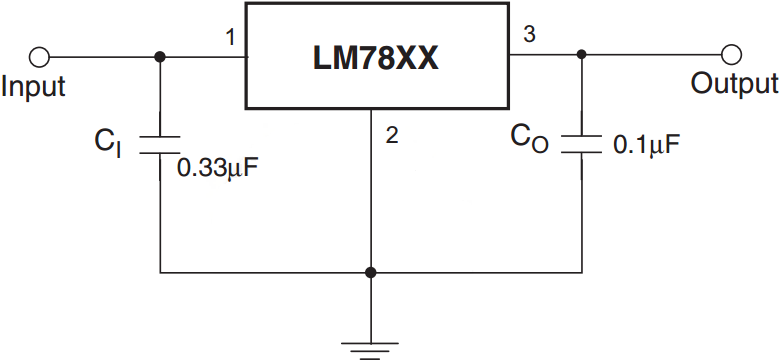
\includegraphics[width=0.4\linewidth]{Hardware/Pictures/LM7805}
	\caption{DC application for LM7805}
	\label{fig:LM7805_app}
\end{figure}

The circuit is built identically as the one seen in the regulator's application note. However, a \SI{1}{\ampere} fuse has been connected to the output in order to protect the supplied circuits from a possible over-current. The final design is seen on Figure \ref{fig:DesignLevelConverter} below.

\begin{figure}[H]
	\centering
	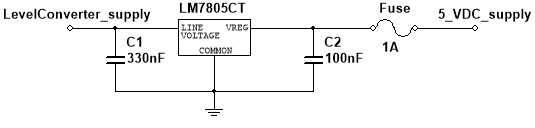
\includegraphics[width=0.7\linewidth]{Hardware/Pictures/DesignLevelConverter}
	\caption{Implemented circuit design on Rolling Road}
	\label{fig:DesignLevelConverter}
\end{figure}

\subsection{Unit test}
The Level Converter is tested using Analog Discovery's built-in oscilloscope. The average output-voltage is found to be \SI{4.97}{\volt}. The output is seen below. \fxnote{Den skal vel testes med den udregnede strøm? (Den bliver godt varm ved det forbrug) - JH}

\begin{figure}[H]
	\centering
	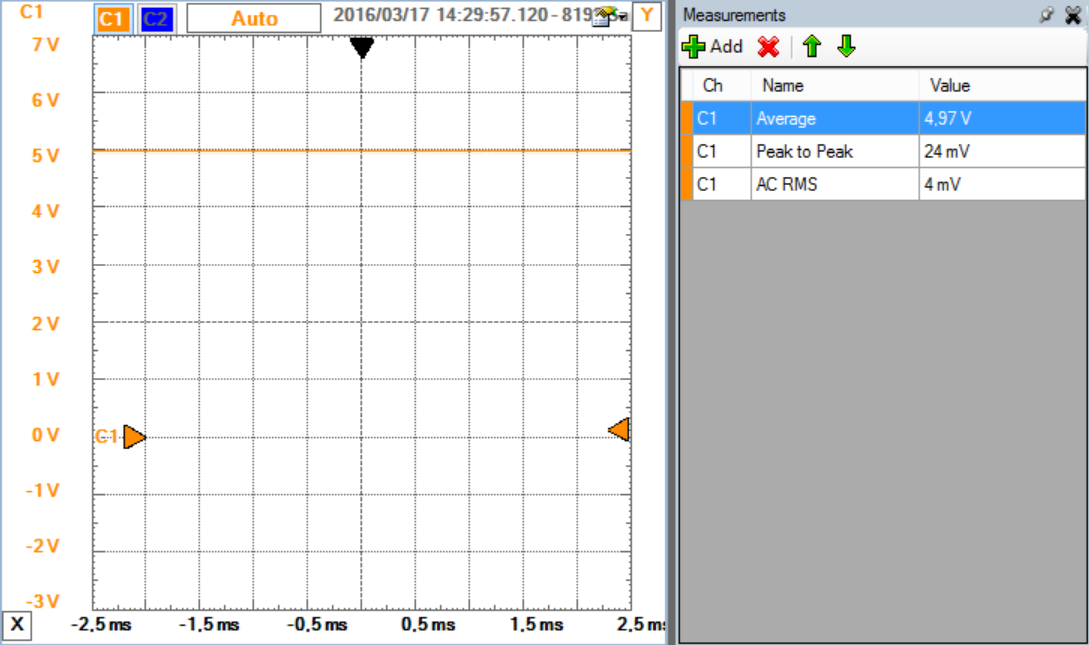
\includegraphics[width=0.9\linewidth]{Hardware/Pictures/LevelConverter_test}
	\caption{Level Converter output over time}
	\label{fig:LevelConverter_test}
\end{figure}